\documentclass[12pt]{article}
\usepackage[a4paper,margin=0.75in]{geometry}
\usepackage[utf8]{inputenc}
\usepackage[OT1]{fontenc}
\usepackage[table,usenames,dvipsnames]{xcolor}
\usepackage{array}
\usepackage{varwidth}
\usepackage{tabularx}
\usepackage{amsmath}
\usepackage{float}
\usepackage{parskip}
\usepackage{hyperref}
\usepackage{forest}
\usepackage{enumitem}
\usepackage{graphicx}
\usepackage{tcolorbox}
\usepackage{forest}

\renewcommand*\familydefault{\sfdefault}

\usepackage{textcomp,    % for \textlangle and \textrangle macros
            xspace}
\newcommand\la{\textlangle\xspace}  % set up short-form macros
\newcommand\ra{\textrangle\xspace}

\definecolor{dkgreen}{rgb}{0,0.6,0}
\definecolor{gray}{rgb}{0.5,0.5,0.5}
\definecolor{mauve}{rgb}{0.58,0,0.82}

\newtcolorbox{mybox}[3][]
{
  colframe = #2!25,
  colback  = #2!10,
  coltitle = #2!20!black,  
  title    = {#3},
  #1,
}

\hypersetup{
    colorlinks=true,
    linkcolor=blue,
    filecolor=magenta,      
    urlcolor=cyan,
    pdftitle={Overleaf Example},
    pdfpagemode=FullScreen,
}

\title{\textbf{Trickle\footnote{The opposite of Torrent :)} : A PSP File Sharing Protocol}}
\author{Aniruddha Deb}
\date{September 2022}

\begin{document}

\maketitle

\tableofcontents

\clearpage

\section{Design}

The design for trickle was guided by three core principles:
\begin{enumerate}
\item \emph{Speed:} The bandwidth should be the bottleneck in file downloads, not the server/client connections, or the software layer
\item \emph{Scalability:} Given a large enough server cache and ample bandwidth/processing power at the server, the server should be able to concurrently service a large number of clients
\item \emph{Reliability:} Irrespective of the Control layer protocol used (UDP or TCP), control messages should achieve their end purpose. This is different from stating all control messages should reach their target: if we don't receive a control message we're expecting, we re-request it until we get it.
\end{enumerate}

More details on how these principles were incorporated are given in the following sections

\subsection{Design Decisions}

Following from above, \emph{C++} was chosen as the language of choice because of it's speed and closeness to the system. Sockets are implemented as syscalls in C, using the POSIX socket library (as a result, this implementation doesn't work on windows). Interfaces were designed in C++ to abstract away the underlying C code for memory safety and portability (more on this in the Code Layout section).

To ensure scalability, \emph{We have to abandon the premise that one client will be serviced by one thread at the server}. Upon having a large number of threads, the OS would spend more time scheduling the threads rather than actually running the threads. This is a well-known, known in systems literature as the \href{https://en.wikipedia.org/wiki/C10k_problem#}{C10K problem} (the ability to concurrently handle 10,000 clients at once).

The solution to this problem is to use a design pattern known as the \href{https://dzone.com/articles/understanding-reactor-pattern-thread-based-and-eve}{Reactor Pattern}: rather than polling the sockets and waiting till we can read/write on them, we assign this task to the kernel. The kernel would then notify us of when a socket can be read to / written from, and we then read/write to the socket at this point. 

\begin{figure}[H]
  \centering
  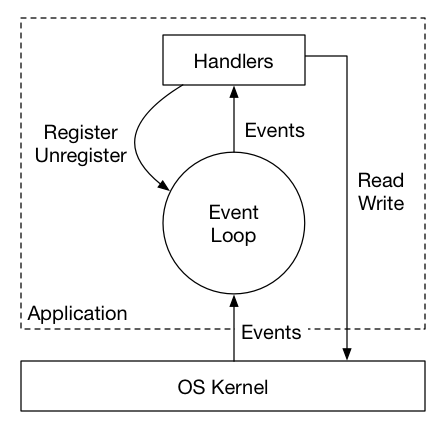
\includegraphics[width=0.5\textwidth]{reactor_pattern.png}
  \caption{The Reactor Design Pattern (Credits: \href{https://teskalabs.com/blog/building-high-performance-application-servers}{TeskaLabs})}
\end{figure}

The Reactor design pattern is implemented in our code using the \href{https://www.freebsd.org/cgi/man.cgi?query=kevent&apropos=0&sektion=0&manpath=FreeBSD+9.0-RELEASE&arch=default&format=html}{kqueue} library. kqueue is the default event queue on MacOS/BSD (my platform), and for other platforms, \href{https://github.com/mheily/libkqueue}{libkqueue} provides a compatiability layer over the underlying event queue library used by the kernel (Linux uses epoll, Windows uses IOCP)

For our third requirement, we register a timer event with our event queue. The timer event triggers a callback every second, and in this callback, we check if there are any stale chunk requests in our buffers (which haven't been responded to by the server). If there are, we clear these requests out and send them again, assuming that they have dropped.

\subsection{Design}

\begin{figure}[H]
  \centering
  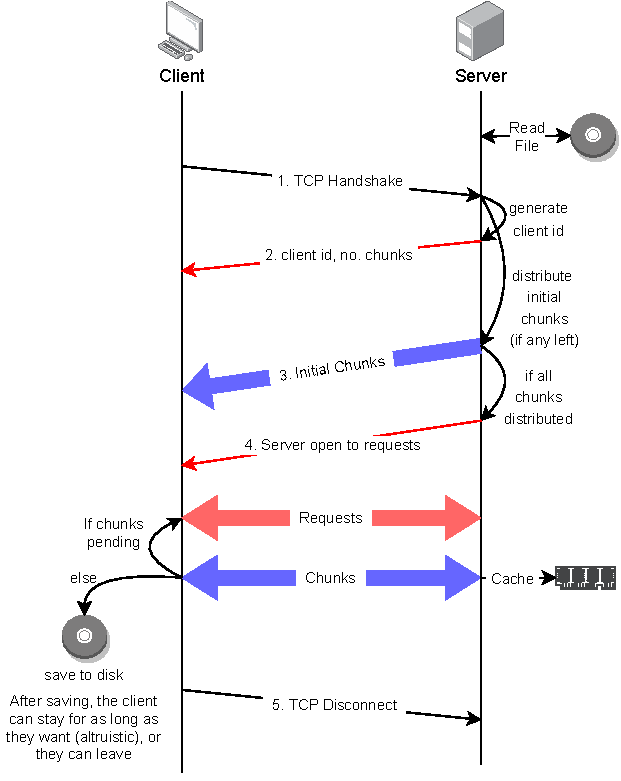
\includegraphics[width=0.6\textwidth]{protocol.pdf}
  \caption{Flow diagram of the trickle protocol (Red - Control layer, Blue - Data layer)}
\end{figure}

Trickle uses two layers: a control layer for sending messages, and a data layer for sending chunks. The protocols used for them vary: Part 1 of the assignment implements the control layer in UDP, and the data layer in TCP, while part 2 does the opposite. We refer to different implementations by \emph{the protocol used for the control layer}. Hence \texttt{server\_udp} represents a server using UDP for control and TCP for data, and \texttt{client\_tcp} represents a client using TCP for control and UDP for data. 

\textbf{The server is implemented Using Only Two Sockets}, one TCP and one UDP, located at the same port of the host machine. Clients are also implemented in the same manner, with both TCP and UDP at the same port. This makes sending messages easier, and keeps the client communicated. The client doesn't need to randomly choose a communication port, and the server doesn't need to keep track of the client addresses at it's various ports. The asynchronous event-loop based structure allows the server to handle multiple clients at once: reads and writes on socket file descriptors are non-blocking, and kqueue informs us of when we can read/write from the socket.

\textbf{Note that both the client and server are asynchronous}: The client does not need to wait for a response to a chunk request to initiate the next chunk request, and neither does the server have to wait for a particular client to reply to a chunk to initiate more chunk requests. This allows for a very fast transfer of data over the network, leaving the burden of sequencing and tabulating the incoming data to the client machine.

\subsection{Protocol}

Two types of messages, Control messages and File Chunks are transferred in the control and data layers respectively. The structure of these chunks is given in fig. 3.

\begin{figure}[H]
  \centering
  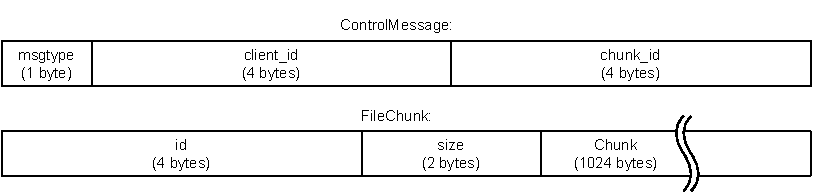
\includegraphics[width=0.9\textwidth]{messages.pdf}
  \caption{Messages used in trickle: ControlMessage and FileChunk}
\end{figure}

The control messages can take the following values:
\begin{center}
\begin{tabular}{|c|c|c|}
\hline
msgtype & client\_id & chunk\_id \\
\hline
REQ     & \la client id \ra & \la chunk id \ra \\
OPEN    &     -     &     -    \\
REG     & \la client id \ra & \la num chunks \ra \\
\hline
\end{tabular}
\end{center}

The FileChunk has 4 bytes for the id, 2 bytes for the size of the data in the chunk and 1024 bytes for the data itself. Note that a chunk can have less than 1024 bytes, if it's the last chunk in the file. For proper reconstruction of the file, the size field is important, as it signifies how many bytes of the data are meaningful.

\subsection{Code Layout}

To accomodate the different implementations, a modular design had to be used: we define three major interfaces, \textbf{Client} (representing the client object), \textbf{Server} (representing the server object) and \textbf{ClientConnection} (representing a connection to a single client on the server side). An overview is given in fig. 4.

\begin{figure}[H]
  \centering
  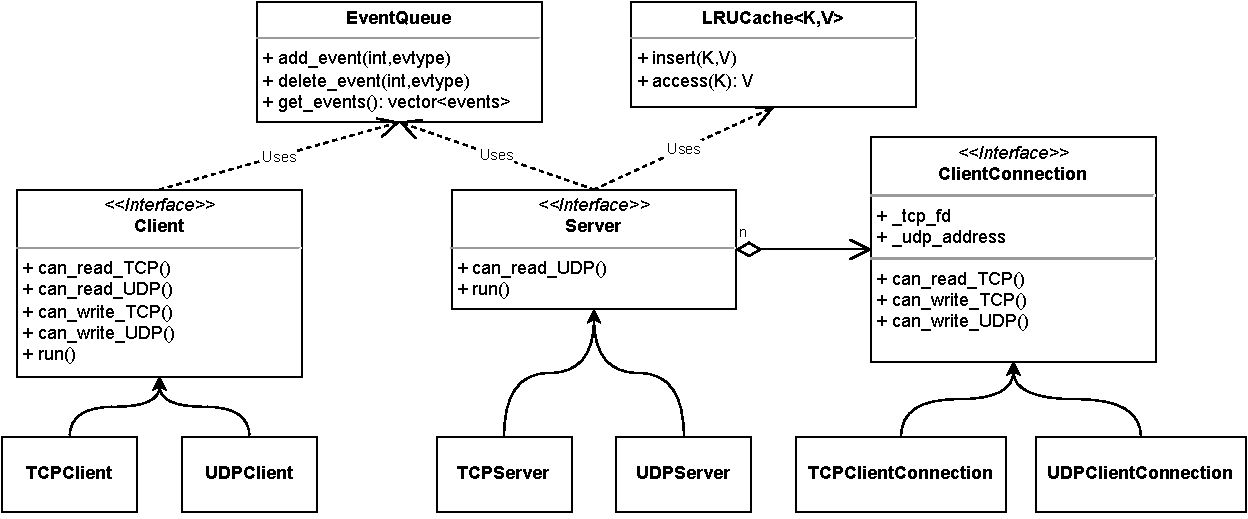
\includegraphics[width=0.9\textwidth]{uml.pdf}
  \caption{UML diagram of the major interfaces and their implementations}
\end{figure}

The interfaces are defined as hpp header files, with code for common implementations defined in the header file itself. The implementation of the specific methods is defined in the \texttt{*\_tcp.cpp} and \texttt{*\_udp.cpp} files. The choice of choosing a TCP or a UDP implementation is made at compile time, by passing the \texttt{PROTO=TCP} flag to the Makefile.

\subsection{Handling Packet Drops}

Packet drops are solely handled by the client side: in case a particular message/chunk drops, the client has a timer that alerts it every second. It will send a request to the server containing the header of the particular message it's expecting for OPEN and REG requests, and will resend the chunk request in case of chunk drops. The timeout for chunk drops is set to be 5 seconds on the client side, and for OPEN and REG misses, is 1 second.

\clearpage

\subsection{Installation and Execution}

\begin{mybox}{red}{NOTE}
The code was tested on Mac (MacOS 10.15.6, g++ v11.2.3) and Linux (Manjaro 21.3, g++ v12.1.1, libkqueue v2.6.1). This program is not compatiable with Windows, and also requires building and installing libkqueue from the GitHub source if on Linux (\texttt{apt-get}/\texttt{pacman} have outdated versions, which have bugs)
\end{mybox}

The files are structured as follows:

{\footnotesize
\begin{forest}
  for tree={
    font=\ttfamily,
    grow'=0,
    child anchor=west,
    parent anchor=south,
    anchor=west,
    calign=first,
    edge path={
      \noexpand\path [draw, \forestoption{edge}]
      (!u.south west) +(5pt,0) |- node[fill,inner sep=1.25pt] {} (.child anchor)\forestoption{edge label};
    },
    before typesetting nodes={
      if n=1
        {insert before={[,phantom]}}
        {}
    },
    fit=tight,
    before computing xy={l=15pt},
  }
[trickle.zip
  [trickle.pdf]
  [trickle.sh]
  [trickle\_proj
    [Makefile]
    [res
      [A2\_small\_file.txt]
    ]
    [src
      [client.hpp]
      [client\_connection.hpp]
      [client\_connection\_tcp.cpp]
      [client\_connection\_udp.cpp]
      [client\_tcp.cpp]
      [client\_udp.cpp]
      [clientmgr.cpp]
      [event\_queue.hpp]
      [lru\_cache.hpp]
      [protocol.hpp]
      [server.cpp]
      [server.hpp]
      [server\_tcp.cpp]
      [server\_udp.cpp]
    ]
  ]
]
\end{forest}
}

The bundled shell script compiles and then runs the code located in \texttt{trickle\_proj}. The executables are generated in \texttt{trickle\_proj/bin}, and the code is run by the script. The \texttt{md5} utility is used to generate a md5sum of the generated files, which are stored in \texttt{trickle\_proj/output}.

\clearpage

\section{Analysis}

\subsection{RTT averages}

The average RTT across all chunks, across all clients for the UDP implementation (Part 1) was \textbf{33423 $\mu$s}. For the TCP implementation (Part 2), the value was \textbf{21011 $\mu$s}. This is when both clients request chunks sequentially, from 0 to $n-1$, and chunks are distributed in a block based manner to all clients (that is, client 0 receives 0..m-1 chunks, client 1 receives 1..2m-1, and so on).

The value for the TCP implementation on average is smaller. This is as expected, as the bulk of the data (that is, the chunks) are transferred over UDP. UDP has no rate limit and no error correction/packet drop protection, hence the client and server can fire away as many chunks as they want over a short period of time. This may lead to congestion (as can be seen in the average RTT across time), but for the small number of clients and chunks here, it is much faster.

\subsection{RTT averages across clients}

\begin{figure}[H]
  \centering
  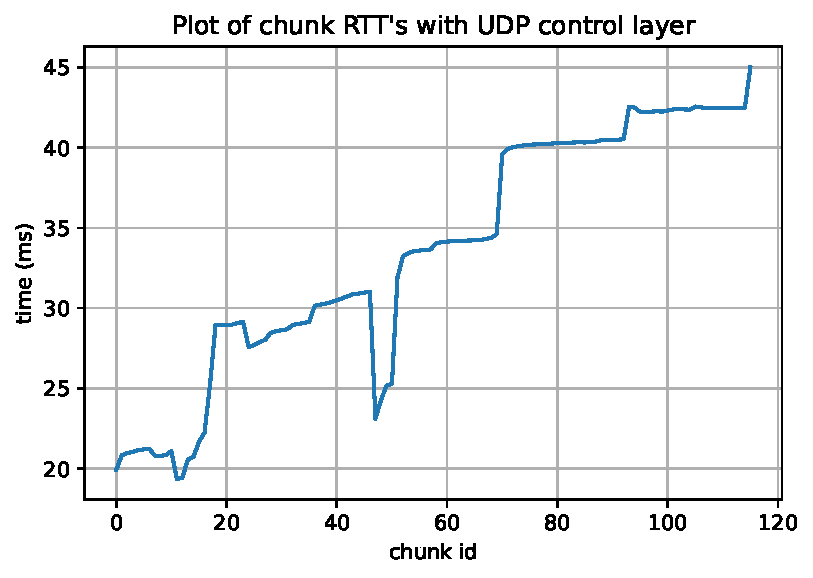
\includegraphics[width=0.49\textwidth]{udp_plot.pdf}
  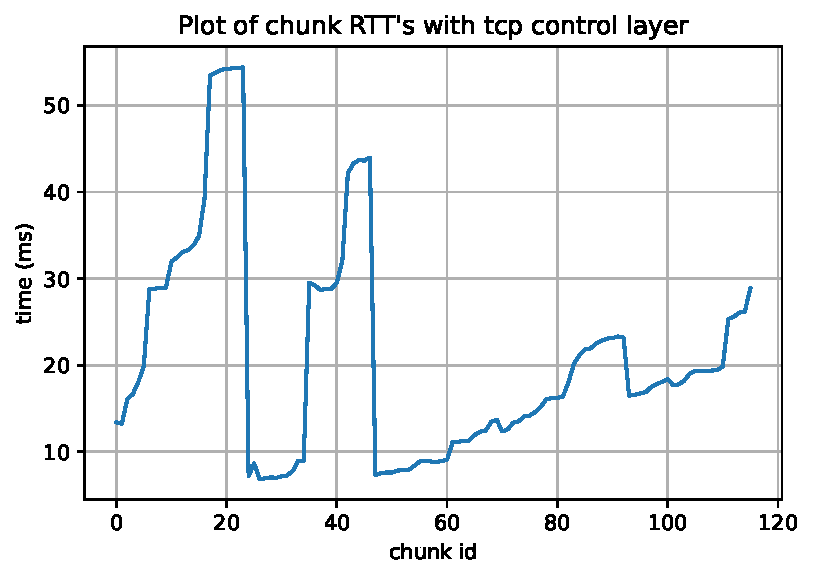
\includegraphics[width=0.49\textwidth]{tcp_plot.pdf}
  \caption{RTT averages for each chunk across clients}
\end{figure}

\begin{itemize}
  \item For the UDP implementation, since chunks are transferred via TCP, we see a monotonic rise in packet request times as we approach the end. As we get to the last chunk, there are more senders of the chunk than receivers, and this generates a lot of congestion on the network. Since TCP has to be reliable and can't drop packets, the time to transmit over this congested network increases.
  \item For the TCP implementation, since chunks are transferred over UDP, there are spikes at chunks 20 and 40: this is because of high demand for a particular chunk. Only one client would have that chunk, and all the four other clients would be demanding that chunk from that particular client, hence the time would increase. Cache misses are also more frequent towards the starting, causing the initial request times to be high.
\end{itemize}

\subsection{Load Benchmark}

\begin{figure}[H]
  \centering
  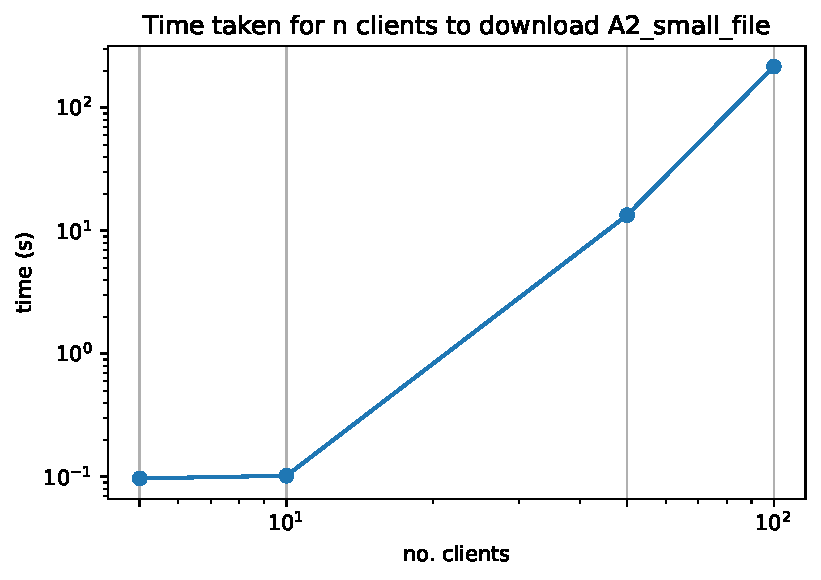
\includegraphics[width=0.6\textwidth]{time_clients.pdf}
  \caption{load statistics with cache size 100. Note that time is recorded from the point the last chunk leaves the server to the point where the last client saves it's file.}
\end{figure}

The load benchmarks are as expected: due to the presence of the central server, as the number of clients increases, the time increases as well (the increase upto 10 clients is not noticeable on a log-scale, due to the fact that there are not enough clients/data being exchanged to generate a bottleneck). For every order of magnitude increase of the number of clients, the time taken increases by three orders of magnitude. 

Note that this increase may also be due to simulation: on my machine, the process simulating the clients took over 95\% of all available resources for $n=100$, leaving only 5\% for the server (each client was simulated using a different thread). A rigorous load benchmark would involve running the server on a network, and having a large set of clients from another machine connect to it.

\subsection{Cache Size Benchmark}

\begin{figure}[H]
  \centering
  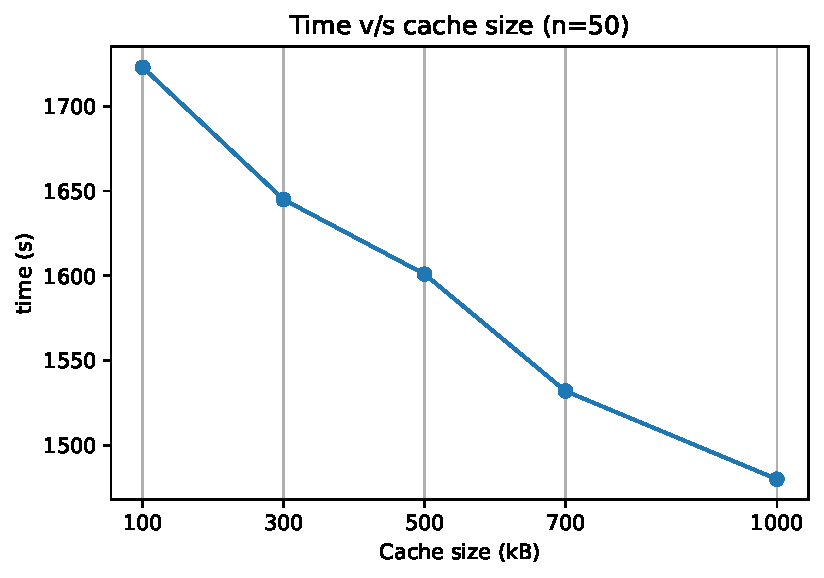
\includegraphics[width=0.6\textwidth]{time_cache.pdf}
  \caption{Time vs cache size plot for 50 clients to download A2\_large\_file.txt}
\end{figure}

Simulating this with a 100 clients on my machine was not possible, as it has only 8GB of memory, and each file takes up 100MB. Since we are not intermittently storing chunks to disk and everything resides in memory, we would need $\sim$ 10GB of memory to simulate this.

Fewer cache sizes as well were simulated: I could only simulate a subset of the initially requested cache sizes, as the time to run the tests was very high (nearing almost 30 min for the longest one). However, the results are in agreement with what is to be expected: \emph{there is a decrease in the total time with an increase in the cache size}. This is because access from cache is faster than going across the network, and a larger cache size implies fewer cache misses. 

The decrease is only marginal: going from 30 minutes to around 24 minutes, because the cache size is still a very small fraction of the total number of chunks. There are $\sim$ 103,000 chunks in the large file, giving us a cache to file ratio of 1:1000 to 1:100. This is too large to have a significant reduction in the time. 

There is also little to no \textbf{Cache Overlap}: Due to the sequential nature of requests and chunk distribution, at any time, the majority of chunks requested would form a window, whose length would be approximately the number of chunks distributed to any one client. Each client gets $\sim$ 2000 chunks in this scenario, while the maximum number of chunks in the cache is only 1000. Hence, by the time we get to a run of chunks that have been requested previously, the cache would contain little to no chunks from that sequence, as they would all have been evicted.

\subsection{Randomized Client Request Sequence Benchmark}

On randomizing the client requests, The process took marginally more time (103 ms compared to 97 ms). This was due to the small number of clients and the speed of the server. However, the average RTT per chunk changed drastically:

\begin{figure}[H]
  \centering
  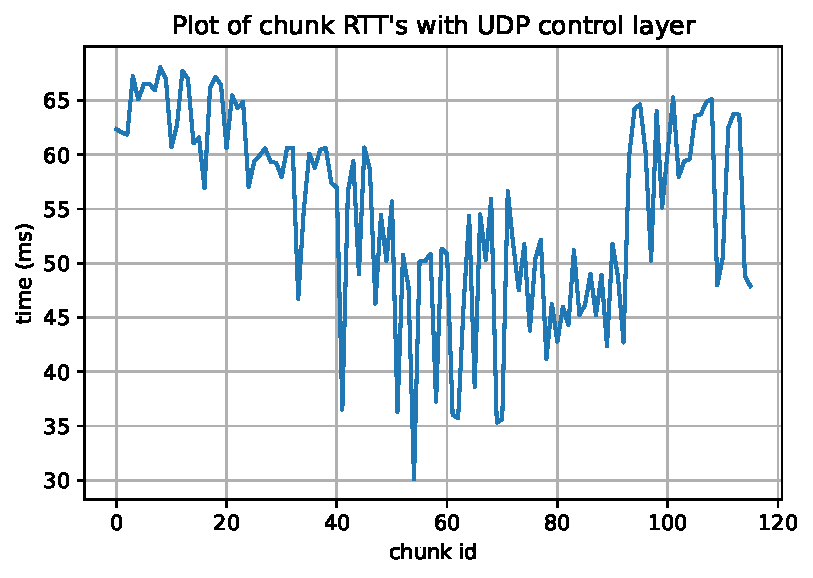
\includegraphics[width=0.6\textwidth]{random_req.pdf}
  \caption{Average chunk response times when requests are random}
\end{figure}

The times are still low, due to the cache size to file ratio, which is 100:116 $\sim$ 0.85. This is a high number, and the random requests have only a 15\% chance of generating a cache miss. As the cache size to file size ratio grows smaller, We expect a randomized request sequence to generate more cache misses, causing the time to shoot up drastically compared to a sequential sequence, where the number of cache hits would be more. 

\end{document}
